%% This is file `elsarticle-template-2-harv.tex',
%%
%% Copyright 2009 Elsevier Ltd
%%
%% This file is part of the 'Elsarticle Bundle'.
%% ---------------------------------------------
%%
%% It may be distributed under the conditions of the LaTeX Project Public
%% License, either version 1.2 of this license or (at your option) any
%% later version.  The latest version of this license is in
%%    http://www.latex-project.org/lppl.txt
%% and version 1.2 or later is part of all distributions of LaTeX
%% version 1999/12/01 or later.
%%
%% The list of all files belonging to the 'Elsarticle Bundle' is
%% given in the file `manifest.txt'.
%%
%% Template article for Elsevier's document class `elsarticle'
%% with harvard style bibliographic references
%%
%% $Id: elsarticle-template-2-harv.tex 155 2009-10-08 05:35:05Z rishi $
%% $URL: http://lenova.river-valley.com/svn/elsbst/trunk/elsarticle-template-2-harv.tex $
%%

%%\documentclass[preprint,authoryear,12pt]{elsarticle}

%% Use the option review to obtain double line spacing
%% \documentclass[authoryear,preprint,review,12pt]{elsarticle}

%% Use the options 1p,twocolumn; 3p; 3p,twocolumn; 5p; or 5p,twocolumn
%% for a journal layout:

%% Astronomy & Computing uses 5p
%% \documentclass[final,authoryear,5p,times]{elsarticle}
\documentclass[final,authoryear,5p,times,twocolumn]{elsarticle}

%% if you use PostScript figures in your article
%% use the graphics package for simple commands
%% \usepackage{graphics}
%% or use the graphicx package for more complicated commands
\usepackage{graphicx}
%% or use the epsfig package if you prefer to use the old commands
%% \usepackage{epsfig}

%% The amssymb package provides various useful mathematical symbols
\usepackage{amssymb}
%% The amsthm package provides extended theorem environments
%% \usepackage{amsthm}

\usepackage[pdftex,pdfpagemode={UseOutlines},bookmarks,bookmarksopen,colorlinks,linkcolor={blue},citecolor={green},urlcolor={red}]{hyperref}
\usepackage{hypernat}

\usepackage{listings}
\usepackage{color}

\definecolor{mygreen}{rgb}{0,0.5,0}
\lstset{
  language=Python,
  basicstyle=\small\ttfamily,
  showstringspaces=false,
  stringstyle=\color{red},
  keywordstyle=\bfseries\color{mygreen},
  morecomment=[l]{/},
  commentstyle=\color{blue},
}

%% The lineno packages adds line numbers. Start line numbering with
%% \begin{linenumbers}, end it with \end{linenumbers}. Or switch it on
%% for the whole article with \linenumbers after \end{frontmatter}.
%% \usepackage{lineno}

%% natbib.sty is loaded by default. However, natbib options can be
%% provided with \biboptions{...} command. Following options are
%% valid:

%%   round  -  round parentheses are used (default)
%%   square -  square brackets are used   [option]
%%   curly  -  curly braces are used      {option}
%%   angle  -  angle brackets are used    <option>
%%   semicolon  -  multiple citations separated by semi-colon (default)
%%   colon  - same as semicolon, an earlier confusion
%%   comma  -  separated by comma
%%   authoryear - selects author-year citations (default)
%%   numbers-  selects numerical citations
%%   super  -  numerical citations as superscripts
%%   sort   -  sorts multiple citations according to order in ref. list
%%   sort&compress   -  like sort, but also compresses numerical citations
%%   compress - compresses without sorting
%%   longnamesfirst  -  makes first citation full author list
%%
%% \biboptions{longnamesfirst,comma}

% \biboptions{}

\journal{Astronomy \& Computing}

%% Make single quotes look right in verbatim mode
\usepackage{upquote}

\begin{document}

\begin{frontmatter}

%% Title, authors and addresses

%% use the tnoteref command within \title for footnotes;
%% use the tnotetext command for the associated footnote;
%% use the fnref command within \author or \address for footnotes;
%% use the fntext command for the associated footnote;
%% use the corref command within \author for corresponding author footnotes;
%% use the cortext command for the associated footnote;
%% use the ead command for the email address,
%% and the form \ead[url] for the home page:
%%
%% \title{Title\tnoteref{label1}}
%% \tnotetext[label1]{}
%% \author{Name\corref{cor1}\fnref{label2}}
%% \ead{email address}
%% \ead[url]{home page}
%% \fntext[label2]{}
%% \cortext[cor1]{}
%% \address{Address\fnref{label3}}
%% \fntext[label3]{}

\title{AST: A library for modelling and manipulating coordinate systems\tnoteref{ascl}}
\tnotetext[ascl]{This code is registered at the ASCL with the code
  entry ascl: \href{http://www.ascl.net/1404.016}{1404.016}}

%% use optional labels to link authors explicitly to addresses:
%% \author[label1,label2]{<author name>}
%% \address[label1]{<address>}
%% \address[label2]{<address>}

\author[jac,eao]{David S.\ Berry\corref{cor1}}
\ead{d.berry@jach.hawaii.edu}
\author[ral]{Rodney F.\ Warren-Smith}
\author[cornell,jac]{Tim Jenness}

\cortext[cor1]{Corresponding author}

\address[jac]{Joint Astronomy Centre, 660 N.\ A`oh\=ok\=u Place, Hilo, HI
  96720, USA}
\address[eao]{East Asian Observatory, 660 N.\ A`oh\=ok\=u Place, Hilo, HI
  96720, USA}
\address[ral]{RAL Space, STFC Rutherford Appleton Laboratory, Harwell Oxford, Didcot, Oxfordshire OX11 0QX, UK}
\address[cornell]{Department of Astronomy, Cornell University, Ithaca,
  NY 14853, USA}

\begin{abstract}
This paper describes the Starlink AST library.
\end{abstract}

\begin{keyword}
%% keywords here, in the form: keyword \sep keyword

%% MSC codes here, in the form: \MSC code \sep code
%% or \MSC[2008] code \sep code (2000 is the default)

WCS \sep data models \sep Starlink

\end{keyword}

\end{frontmatter}

% \linenumbers

%% Journal abbreviations
\newcommand{\mnras}{Mon Not R Astron Soc}
\newcommand{\aap}{Astron Astrophys}
\newcommand{\aaps}{Astron Astrophys Supp}
\newcommand{\pasp}{Pub Astron Soc Pacific}
\newcommand{\apj}{Astrophys J}
\newcommand{\apjs}{Astrophys J Supp}
\newcommand{\qjras}{Quart J R Astron Soc}
\newcommand{\an}{Astron.\ Nach.}
\newcommand{\ijimw}{Int.\ J.\ Infrared \& Millimeter Waves}
\newcommand{\procspie}{Proc.\ SPIE}
\newcommand{\aspconf}{ASP Conf. Ser.}

%% ASCL
\newcommand{\ascl}[1]{\href{http://www.ascl.net/#1}{ascl:#1}}

%% main text
\section{Introduction}
\label{sec:intro}

The Starlink AST library \citep[][\ascl{1404.016}]{SUN211} provides a
generalised scheme for modelling, manipulating and storing inter-related
coordinate systems. Whilst written in C, it has bindings for several
other languages including Python, Java, Perl and Fortran. It has
specialised support for many of the coordinate systems and projections
commonly used to describe astronomical World Coordinate Systems (WCS),
including all those described by the FITS-WCS standard, plus various
popular distortion schemes currently in use. However, it is not limited
to WCS, and may be used in any situation requiring transformation between
different coordinate systems.

Unlike FITS-WCS, which supports only a relatively small set of prescribed
transformation recipes reflecting the coordinate transformations within
an optical telescope, AST allows arbitrarily complex transformations to be
constructed by combining simple atomic transformations in series or in
parallel. This allows a much wider range of transformations to be
described than is possible using FITS-WCS, and so can accomodate a wider
range of data storage forms without the need to re-grid the data.

AST was released internally in 1997 \cite[][included in ``Twenty Years of
ADASS'' \nocite{adass20}]{1998ASPC..145...41W}. Since then it has been in
continuous use within the Starlink Software Collection \citep[][\ascl{1110.012}]{2014ASPC..485..391C}
and is also used by various other major astronomical software tools such as
DS9 \citep[][\ascl{0003.002}]{2003ASPC..295..489J}. Interest in flexible schemes for representing
inter-related coordinate systems has increased recently\footnote{For
instance, in the discussions about possible succesors to the FITS format \citep{2015Mink},
and within the Astropy project \citep{2013A&A...558A..33A}}, and so it seems an appropriate time to
review the lessons learned from AST.

This paper first presents an account of the historical issues that drove
the initial development of AST, together with the reasoning behind some
of the design decisions, and then presents an over-view of the more
important aspects of the data model used by AST.

\section{Historical Perspective}

\subsection{Initial Problems}

The first public release of the AST library was in 1998
\citep{1998StarB..20....6L,1998StarB..20....7D} but some of the
underlying concepts date from the late 1980s, when the Starlink
Project was designing its NDF data format for gridded astronomical
data \citep{2015Jenness}. There was clearly a need to relate positions
within gridded data, using coordinates based on pixel indices, to
real-world positions on the sky, wavelengths in a spectrum and so
on. These non-pixel coordinate systems are now generally known as
world coordinate systems (WCS).

Calibration of spectra, for example, was commonly performed by fitting
a polynomial to express wavelength as a function of pixel position and
then either storing the polynomial coefficients, or tabulating the
polynomial value at each pixel centre. While not completely general,
the latter option was an acceptable solution and was adopted as part
of the Starlink data format. An array giving the central wavelength at
each pixel was stored as the \texttt{AXIS} component in the NDF data
structure and did good service in spectroscopic applications. It was
also possible, in a simple minded way, to attach an \texttt{AXIS}
array to each dimension of an image or any gridded dataset of higher
dimensionality. This allowed each of its axes to be calibrated in
terms of world coordinates.

This approach was adequate if the axes represented independent
quantities (like wavelength and position for a long-slit spectrum),
but did not suffice if the axes were inter-independent. Unfortunately,
in the common case of celestial coordinates (such as Right Ascension
and Declination), the axes are almost always inter-dependent. This is
because the sky is essentially spherical and its coordinates are
therefore naturally curvilinear when projected into two
dimensions. This inter-dependence is a common feature of world
cordinate systems in practice, so a solution was clearly needed that
addressed it properly.

The Flexible Image Transport System
\citep[FITS;][]{1981A&AS...44..363W,1995ASPC...77..233G}, at that
time, addressed the issue in a better but still rudimentary way. In
essence, it stored a physical pixel size (e.g., in seconds of arc),
allowed for a linear scaling of an image (typically to allow for the
position angle rotation of the telescope) and then projected it on to
the celestial sphere using one of a defined set of map
projections. This representation was clearly based on a model of a
physical telescope and how it imaged an observed region of the sky in
its focal plane.

While successfully accommodating the curvilinear nature of sky
coordinates, this FITS approach was still limited in many ways. In
essence, it defined a small set of functional forms (based on map
projections) through which pixel coordinates could be mapped on to
celestial coordinates and back again. However, if the actual
relationship between pixel coordinates and world coordinates didn't
correspond to one of these functional forms, then it wasn't possible
to use FITS to store the coordinate information\footnote{Unless the data was
first re-gridded into a form supported by FITS.}.

For instance, if astronomical instrumentation were to use a novel map
projection, if arbitrary instrumental distortions were present or if
the data were re-gridded into a non-physical space, then the FITS
approach would fail. It also had limited support for high-accuracy
astrometry, where the departure of the sky from a perfect sphere, for
a variety of reasons, has to be taken into account. In addition, there
are many other non-celestial world coordinate systems that one might
use (involving energy, velocity, time, frequency, \emph{etc}.) that no
contemporary system could represent adequately.

Unfortunately, this list of limitations only scratches the surface of
the problem as it was perceived at the time. Other considerations,
such as the time-dependent relationship between non-inertial celestial
coordinate systems, the dependence of apparent positions on the
position and velocity of the observer (and also on the wavelength of
observation and atmospheric conditions) and periodic revisions to the
fundamental definitions of celestial coordinate and time systems would
all have to be accommodated, as would numerous other issues specific
to particular domains (celestial coordinates, time systems, radial
velocities, wavelength/energy, \emph{etc}.). This was several years before the
FITS community commenced work on what was eventually to become the current
FITS-WCS standard.

\subsection{TRANSFORM}

In the late 1980s, no immediate and general solution to these problems
could be seen. Recognising the limitations in the FITS approach,
however, the Starlink Project decided to take a hard line and to omit
completely any component dedicated to world coordinate systems from
its new NDF data format. Instead, this \emph{astrometry extension}
(from which the name AST is derived) was to be added at a later date
when a suitable solution had been formulated.

This decision was undoubtedly strongly influenced by Patrick Wallace's
presence in the Project and the major work he had done on the SLALIB
library \citep[][\ascl{1403.025}]{1994ASPC...61..481W} to encapsulate best-practice in
astrometric calculations (and also in other domains such as time
systems). Discussion within the Project rapidly convinced us that if
we adopted the FITS approach as it existed at the time, we would cut
ourselves off from the proper rigorous treatment of astrometric data
that is needed for the highest accuracy.

Consequently, a pilot project was conducted to explore alternative
approaches. The most important limitation of the FITS approach was felt
to be the use of a fixed set of functional forms (map projections) each
of which was associated with a small fixed set of parameters. This
simplified storing the information in 80-character FITS \emph{header cards},
but clearly the set of functional forms that might ultimately be needed
was much larger than had been recognised. Adding new ones might become a
never-ending project and that, in turn, raised the prospect of
continually upgrading all software that had to read and process FITS
headers and handle coordinate systems.

The alternative approach that we explored was to write an expression
parser that would accept sets of arithmetic expressions similar to those
used in Fortran and C, along with the usual set of mathematical
functions. Together with a method of passing named parameter values into
these expressions, this greatly increased the set of functional forms
that could be represented. The expressions themselves (encoded as
character strings) and the associated parameter values could easily be
stored in astronomical datasets. Typically, one set of expressions would
relate pixel coordinates to world cordinates (e.g. sky coordinates) and
a second, optional, set would define the inverse transformation. The
expression syntax was powerful enough to represent a wide range of map
projections plus many other transformations into alternative world
coordinate systems.

A processing engine was also provided that could use the stored
expression data to transform actual coordinate values.

A library implementing this, called \textsc{transform}, was released
in 1989 \citep{SUN61,1989StarB...4....7L}. It stored its data (the
expressions and parameters) in Starlink's Hierarchical Data Format
\citep[HDS;][]{SUN92,SSN27,2015HDS} and was thus able to integrate with the
Starlink NDF data format to attach arbitrary world corrdinates to
gridded astronomical datasets.


\subsection{TRANSFORM Lessons}

Ultimately, \textsc{transform} turned out not to be a full solution to
the WCS problem and did not become part of the NDF data
format\footnote{Although it it was the precursor of the
  \texttt{MathMap} class in AST.}. It was, however, used for two
initially unforeseen purposes which turned out to be very significant:

\begin{enumerate}
\item Associating coordinate systems with plotting surfaces in a
  ``graphics database'' \citep[see e.g.,][]{SUN48}. This allowed
  plotting applications to store a coordinate system for (say) a graph
  plotted in logarithmic coordinates so that those coordinates could
  later be recovered from the position of a cursor. This demonstrated
  that plotting was a major application area for this type of
  technology, especially when using curvilinear coordinates such as
  Right Ascension and Declination which are notoriously difficult to
  handle properly with standard plotting software.

\item Transformation and combination of bulk image data using general
  arithmetic expressions (as an alternative to combining images using
  a manual sequence of add/subtract/multiply/divide and similar
  applications). This showed that (a) the approach could easily be
  efficient enough to handle large datasets and (b) the data values in
  an image were just another coordinate that could be transformed into
  different representations (logarithmic, different units, \emph{etc}.) in
  much the same way as its axes.
\end{enumerate}

With these insights, it was clear that the ideas behind
\textsc{transform} had potential, but some serious deficiencies had
also emerged:

\begin{itemize}

\item Arithmetic expressions, while fairly general, could not easily
  cope with coordinate transformations that required iterative
  solution, nor with discontinuous transformations, nor with look-up
  tables or a variety of other computational techniques. While
  arithmetic expressions provided a valuable increase in the
  flexibility of coordinate transformations, clearly other classes
  were still needed.

\item It was a major problem for the average writer of astronomical
  software to formulate the required coordinate expressions correctly
  even when dealing with quite simple sky coordinate systems. The core
  of this issue is that celestial coordinate systems are rather
  complex and a good deal of specialist knowledge is needed to
  formulate even simple cases correctly. Clearly a better solution
  would be to encapsulate this knowledge in the WCS software and
  provide a simpler API that dealt only in high-level concepts.

\item For high accuracy work, further complex calculations
  arise. These are related, for example, to atmospheric refraction and
  special \& general relativistic effects (like the observer's motion
  and the sun's gravity).  These require the use of a dedicated
  library of astrometric functions and cannot in practice be handled
  by simple expressions. They also require additional data about the
  observing context (time, position, velocity, wavelength, \emph{etc}.) and
  any practical solution must define how these are stored and
  processed.

\item \textsc{transform} had no ability to store additional
  information about data axes, such as labels and units.

\item It became clear that coordinate transformations frequently
  needed to be combined, for example by applying one transformation
  after another, and that this process was often inefficient. The key
  to better efficiency lay in knowing more about each transformation,
  like whether it was linear or had a variety of other
  properties. With this information it was possible to merge (or
  cancel out) consecutive transformations for better
  efficiency. \textsc{transform} had a rudimentary system for encoding
  this information, but it was not really up to the task.

\item Tying WCS software to a particular (Starlink) data system was a
  mistake and limited the uses to which it could be put. It would
  clearly be better if the data could be encoded (serialised) in
  alternative ways to make it data-system agnostic. The same
  agnosticism should also apply to other likely dependencies, like
  graphics systems and error reporting.  The ability to implement
  these services in alternative ways would be especially important
  when designing graphical user interfaces that processed WCS
  information.

\end{itemize}

\subsection{Developments in FITS WCS}

At about the same time, the wider FITS community also came to recognise
some of the limitations of WCS handling within FITS, and in 1992 work commenced
on a new standard for storing WCS information within FITS files. However,
in view of the ``once FITS, always FITS'' principle, that work consisted
mainly in formalising and extending existing practices. So for instance, new
keywords were defined to store the extra meta-data needed for a complete
description of a celestial coordinates system, and new projection types were
added, but the basic model remained unchanged. The new standard still required
that the transformation be split into three components applied in series; an
affine transformation that converts pixel coordinates into \emph{intermediate
world coordinates}, a spherical projection that converts these into \emph{native
spherical coordinates}, and a spherical rotation that converts these into the
final world coordinate system.

In view of the decision to stay with this rigid and restrictive model,
and in view of expected length of time needed to agree a new standard\footnote{An
expectation that was justified when the standard was finally published in 2002.},
the Starlink project decided in early 1996 to develope its own WCS system, informed
by the earlier experiments with \textsc{transform}, rather than adopt the new FITS
standard.

\subsection{AST Principles}

One of the first decisions was to
separate the representation of a coordinate system (that we called a
Frame) from the computational recipe that transforms between
coordinate systems (a Mapping). From the \textsc{transform} experience
we knew we would need multiple classes of both these data types, all
of which would need to support the same basic operations, but each
having its own specialisation. The correspondence with sub-classing in
object-oriented (OO) programming was irresistible and the decision to
use an OO design immediately followed.

This raised the issue of an implementation language. We planned to use
the SLALIB library for astrometric calculations\footnote{A later version
of AST eventually replaced SLALIB with SOFA and PAL.}. This had been
developed with extreme portability in mind and had recently been
re-written in ANSI C. We didn't want to compromise this portability,
so decided also to work in strict ANSI C and to minimise software
dependencies as much as possible. This meant providing portable
interfaces to facilities that were intrinsically less portable, such
as data file access, plotting, error reporting, \emph{etc}. and providing
simple implementations that users could re-write if necessary.

Deciding to write an OO system in a non-OO language took considerable
thought. We needed to provide a Fortran-callable interface but, at the
time, the portability of C++ code was quite limited if one needed to
call it from Fortran, so that route was unattractive. Eventually, we
were guided by the approach described by \citet{1992Holub} for
handling objects in C and were able to hide the detail from users
using pre-processor macros.

One consequence of this is that users cannot easily create new
sub-classes from AST objects without learning the internal conventions
that it uses. At the time, this was seen as something of an advantage.
The library is intended for data interchange and creating new
sub-classes would inevitably allow persistent objects to be created
that other users could not access. However, with hind-sight a more open
architecture may have encouraged involvement from a wider user-base.
\footnote{For Mappings, where this
  issue is most relevant, the problem has been mitigated in a
  controlled way by the IntraMap class that allows separately-compiled
  code to be imported into the library.}.

As noted previously, we wanted the AST API to deal in high-level
concepts and to hide as much specialist detail as possible from the
user. This principle arose from considering the complex calculations
involved in handling celestial coordinates and time systems. However,
we soon realised that two other areas were similarly complex and could
benefit from the same approach.

The first area was graphics. Plotting in curvilinear coordinates is a
complicated business if one wants to handle all the corner cases
correctly. Plotting and labelling celestial coordinate axes, for
example, presents many problems; especially near the poles of an all-sky
projection. It is made even harder if the projection contains
discontinuities. But the high-level concepts involved in such plotting
(coordinate systems and the mappings between them) are such a natural
fit with other AST concepts that it seemed obvious to implement a class
of coordinate system that is specialised for graphics. The high-level
operations it supports would then hide the details of the complex and
generalised plotting algorithms involved.

The second area is an aspect of data storage -- namely the handling of
FITS header cards. While the AST library could provide ways to
serialise its own data transparently, possibly in multiple ways, it
also needed to inter-operate with FITS. WCS data in FITS data files is
stored in a series of 80-character header cards and, over the years,
the number of different ways the information can be stored in these
headers has grown. The complexity involved is now considerable
\citep[see e.g.,][]{2015Thomas}. Again, detailed specialist knowledge
is needed to extract this information reliably and to write it back
(possibly modified) in a form that gives other FITS-handling software
a chance of using it while not conflicting with the many other FITS
headers typically present.

For a user of the AST library, we wanted this process of accessing FITS
headers to appear as much like a simple read/write operation as
possible, with all the implementation details hidden. This requirement
arose from more than simply ease-of-use. FITS header conventions (many
of them informal) are in constant flux and if these details are embedded
in applications programs, those programs must constantly receive
attention if they are to remain up to date. Embedding all these details
in the AST library allows the problem to be addressed in one place and
by someone with the necessary expertise.

FITS header handling has proved one of the most complex areas to tame in AST.
But introducing the concept of a \emph{destructive read} (which reads WCS
data from FITS headers and simultaneously deletes the relevant headers)
has made it possible to write applications with very little code that
have completely general handling of FITS WCS headers.


\section{The AST Data Model}
\label{sec:model}

The most basic principle behind the AST data model is a clear distinction
between a \emph{transformation} and a \emph{coordinate system}.

A \emph{transformation} is a mathematical recipe for converting a numerical
input vector into a corresponding numerical output vector. The
transformation itself has no knowledge of what the values within these
vectors represent, other than that each one constitutes a position within
some unspecified N-dimensional space\footnote{The dimensionality of the
output space need not be the same as that of the input space.}.

A \emph{coordinate system} is a collection of meta-data describing a set of
one or more axes. This will include:
\begin{itemize}
\item the number of axes (i.e. dimensionality of the space)
\item the physical quantity described by each axis
\item the units used by each axis
\item the geometry of the space that they describe (flat, spherical,
\emph{etc})
\item the nature of the coordinate system (Cartesian, polar, \emph{etc})
\item other meta-data that may be needed to specify the coordinate system
fully.
\end{itemize}

These two concepts are encapsulated within two separate classes in the
AST data model: the \emph{Mapping} class and the \emph{Frame} class. This
separation underlines the fundamental difference between the two main
requirements of any coordinate handling system:

\begin{enumerate}
\item knowing \emph{how} to convert numerical positions from one coordinate
system to another.
\item knowing \emph{what} those coordinate systems represent.
\end{enumerate}

As an example of how this distinction is applied in practice, the
\emph{pixel size} of a typical 2-dimensional image of the sky is
\emph{not} considered to be a property of the (RA,Dec) Frame, since it is
determined by the nature of the transformation from pixel coordinates to
(RA,Dec) coordinates, rather than being an intrinsic property of the (RA,Dec)
coordinate system itself.

The two base classes, \emph{Mapping} and \emph{Frame}, are extended
to create a wide variety of sub-classes, each of which describes a
specific form of transformation or coordinate system. New sub-classes can
be added as required and slot naturally into the existing
infra-structure provided by the rest of AST.

In addition, this separation into two ``orthogonal'' classes makes it
easy to create complex compound objects from simple component objects.
For instance, multiple Mappings can be combined into a new object, and
the resulting object will itself be a Mapping. Likewise, multiple Frames
can be combined into a new object, and the resulting object will itself be
a Frame\footnote{For instance, an 2-dimensional (RA,Dec) Frame can be
combined with a 1-dimensional wavelength Frame to create a 3-dimensional
(RA,Dec,Wavelength) Frame.}.

However, at some point these two classes need to be brought together to
provide a complete description of a set of related coordinate systems.
The \emph{FrameSet} class is used for this purpose. A \emph{FrameSet}
encapsulates a collection of two or more Frames, with the Mappings that
describe the transformation between the corresponding coordinate systems.
The simplest FrameSet contains two Frames, together with a single Mapping that
describes how to convert positions between these two Frames (see
Fig.~\ref{fig:simple-frameset}).

\begin{figure}[h]
\centering
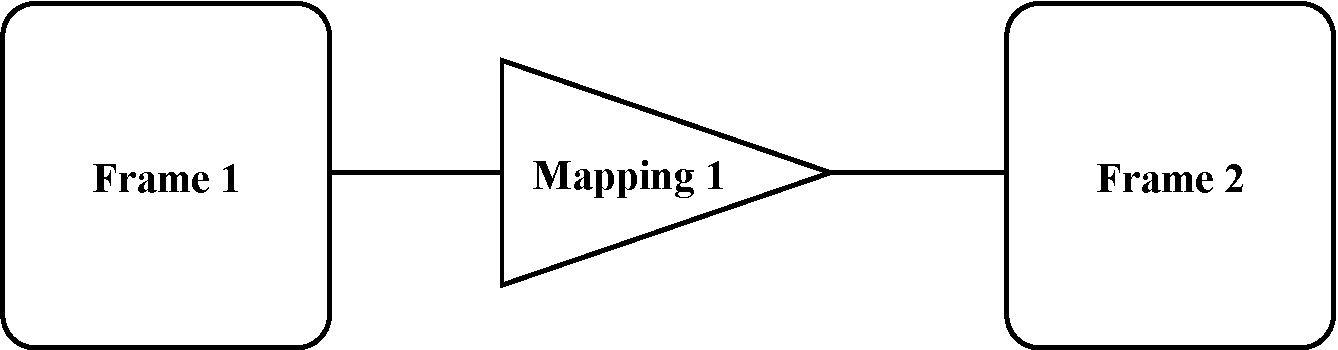
\includegraphics[width=0.5\columnwidth]{simple-frameset}
\caption{A FrameSet that describes two coordinate systems and the
transformations between them. The Mapping's \emph{forward} transformation
transforms positions in \emph{Frame 1} to the corresponding position in
\emph{Frame 2}. The Mapping's \emph{inverse} transformation
transforms positions in \emph{Frame 2} to the corresponding position in
\emph{Frame 1}. }
\label{fig:simple-frameset}
\end{figure}

More complex FrameSets can be created that describe the relationships between
multiple Frames in the form of a tree structure (see
Fig.~\ref{fig:complex-frameset}).

\begin{figure}[h]
\centering
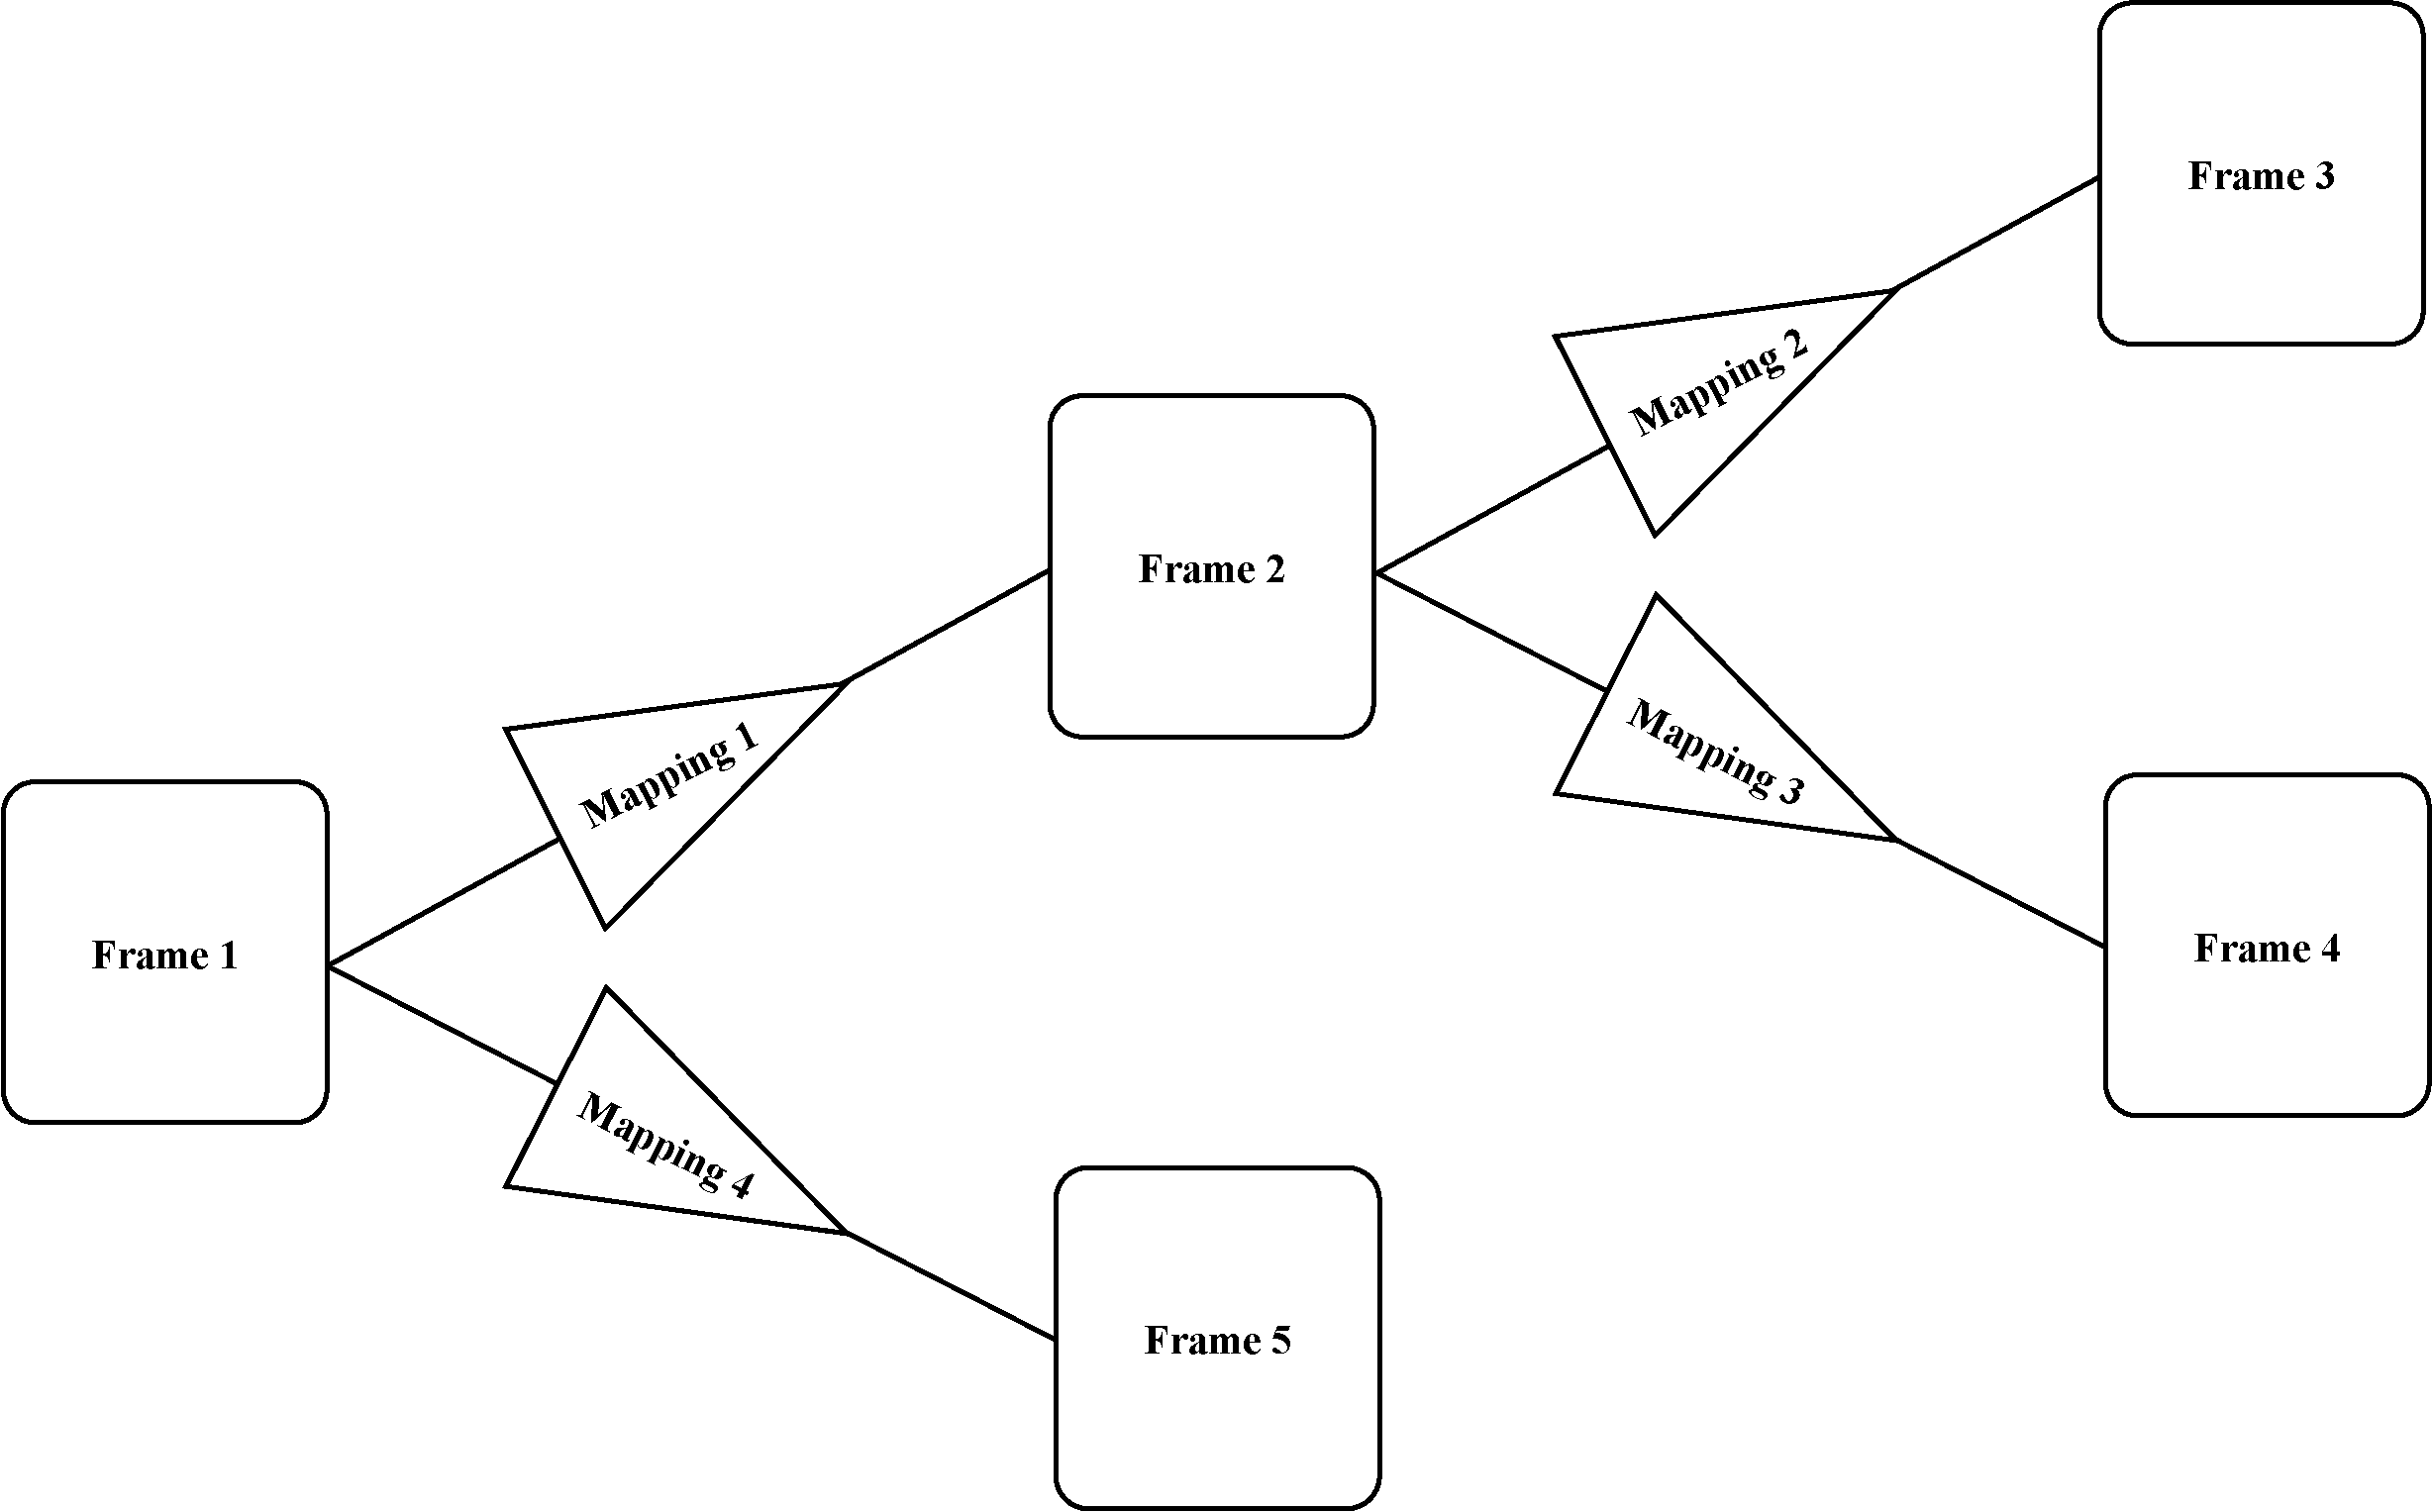
\includegraphics[width=\columnwidth]{complex-frameset}
\caption{A FrameSet that describes five inter-related coordinate systems
and the transformations between them. }
\label{fig:complex-frameset}
\end{figure}

A selection of the more significant methods and properties of these
three classes are described in appendix~\ref{app:classes}.

\subsection{Transformations and Mappings}
Within AST, most \emph{Mappings} encapsulates two transformations - one is
designated as the \emph{forward} transformation and the other as the
\emph{inverse} transformation. When a Mapping is used to transform a set
of positions, the caller must indicate if the forward or inverse
transformation is to be used. The \emph{forward transformation} converts
positions within the input space of the Mapping into corresponding
positions within the output space, and the \emph{inverse transformation}
converts positions within the output space of the Mapping into corresponding
positions within the input space. A Mapping can be \emph{inverted}, which
results in the two transformations being swapped.

For most classes of Mapping, the inverse transformation is a genuine
mathematical inverse of the forward transformation. However, this is not
an absolute requirement, and there are a few classes of Mapping where
this is not the case (for instance the \emph{PermMap} class, in which the
axes of the output space are a permuted subset of the axes of the input
space). In addition, the Mapping class does not require that \emph{both}
transformations are defined. For instance, the \emph{MatrixMap} class, which
multiplies each input vector by a specified matrix to create the output
vector, will only have an inverse transformation if the matrix is square
and invertable.

\subsubsection{Classes of Mapping Provided by AST}
AST provides many classes of Mapping that implement a wide range of
different transformations. Most of these are \emph{atomic} Mappings that
implement a specific numerical transformation and, if possible, its inverse.
But some are \emph{compound} Mappings that combine together other Mappings
(atomic or compound) in various ways to create a more complex Mapping.
A compound Mappings does not define its own transformations, but instead
inherits the transformations of the individual component Mappings which
it encapsulates.

The most significant atomic Mapping classes are:

\begin{description}
\item[UnitMap:] Copy positions from input to output without any change.
\item[WinMap:] Transform positions by scaling and shifting each axis.
\item[ZoomMap:] Transform positions by zoom all axes about the origin.
\item[ShiftMap:] Translate positions by adding an offset to each axis.
\item[MatrixMap:] Transform positions using a matrix.
\item[PolyMap:] A general N-dimensional polynomial transformation.
\item[PermMap:] Transform positions by permutating and selecting axes.
\item[LutMap:] Transform 1-dimensional coordinates using a look-up table.
\item[MathMap:] Transform coordinates using general algebraic mathematical expressions.
\item[WcsMap:] Implements a wide range of spherical projections.
\item[SlaMap:] Transforms positions between various celestial coordinate systems.
\item[SpecMap:] Transforms positions between various spectral coordinate systems.
\item[SphMap:] Map 3-d Cartesian to 2-d spherical coordinates.
\item[TimeMap:] Transforms positions between various time coordinate systems.
\item[PcdMap:] Apply 2-dimensional pincushion/barrel distortion.
\item[DssMap:] Map points using Digitised Sky Survey plate solution.
\item[GrismMap:] Models the spectral dispersion produced by a grism.
\item[IntraMap:] Map points using an externally supplied transformation function.
\item[SelectorMap:] Locates positions within a set of Regions (see
section~\ref{sec:cmpmap}).

\end{description}

The most significant compound Mapping classes are (see
section~\ref{sec:cmpmap} for a more detailed explanation of some of these
classes):

\begin{description}
\item[CmpMap:] Combines two encapculated Mappings in series or parallel.
\item[SwitchMap:] Selects from a set of alternate Mappings depending on
the location of each input position.
\item[TranMap:] Use the forward transformations from one Mapping and the
inverse transformation from another.
\item[RateMap:] A Mapping that represents an element of the Jacobian
matrix of an encapsulated Mapping.
\end{description}

All classes of Mapping are immutable. That is, a Mappng cannot be changed
once it has been created. This is unlike Frame and FrameSet objects, which
\emph{can} be changed.

\subsubsection{Compound Mappings}
\label{sec:cmpmap}

The CmpMap class is a subclass of Mapping that encapsulates two other
Mappings either in series or in parallel. Either or both of the two
encapsulated Mappings can itself be a CmpMap, allowing arbitrarily complex
Mappings to be created.

In a \emph{series} CmpMap, each input position is transformed by the
first component Mapping, and the output from that Mapping is then
transformed by the second component Mapping. Consequently, the output
dimensionality of the first Mapping must be the same as the input
dimensionality of the second Mapping.

In a \emph{parallel} CmpMap, the input space is split into two subspaces.
The first component Mapping is used to transform the axis values
corresponding to the first subspace, and the second component Mapping is
used to transform the axis values corresponding to the second subspace.
Thus the input dimensionality of the CmpMap is equal to the sum of the
input dimensionalities of the two component Mappings, and the output
dimensionality of the CmpMap is equal to the sum of the output
dimensionalities of the two component Mappings.

The SwitchMap class is a subclass of Mapping that allows a different
transformation to be used for different regions within the input space.

Each SwitchMap encapsulates any number of other Mappings, known as ``route''
Mappings, and one ``selector'' Mapping. All of these Mappings must have the
same input dimensionality, and all the route Mappings must have the same
output dimensionality. The selector Mapping must have a one-dimensional
output space.

Each input position supplied to the SwitchMap is first transformed by the
selector Mapping. The scalar output from the selector Mapping is used to
index into the list of route mappings. The selected route mapping is then
used to transform the input position to generate the output position
returned by the SwitchMap.

There is a specialised subclass of Mapping, the SelectorMap class, that
is designed specifically to fulfill the role of the selector Mapping
within a SwitchMap, but in principle \emph{any} suitable form of Mapping
may be used. The SelectorMap class encapsulates several Regions (see
section~\ref{sec:region}) and returns an output value that indicates
which of the  Regions (if any) contained the input value. Thus, the
SwitchMap would typically contain one route Mapping for each of the
Regions contained within the SelectorMap.

\subsubsection{Simplification}
\label{sec:simplification}

There are a wide range of possible transformations that could
potentially be applied to a data set during analysis. These
including simple things such as rotation, scaling, shear, \emph{etc}., but
could in principle include more complex transformations such as
re-projection, dis-continuous ``patchwork'' transformations, or even
transformation using a general algebraic expression.  A coordinate
handling system should make it possible for a user to apply an
arbitrary set of such transformations in series to a data set, without
losing track of the coordinates of each data point. With a
prescriptive scheme such as FITS-WCS this would require each
transformation to locate the appropriate component of the FITS-WCS
pixel to world coordinate mapping, and modify the corresponding
headers in a suitable way. This is often a difficult, if not
impossible, task. Within AST, the chaining of transformations is
accomplished simply by creating a Mapping that describes each new
transformation and concatenating it with the existing pixel to world
coordinate mapping by creating a new CmpMap (see section~\ref{sec:cmpmap}).

However, by itself this can lead to Mappings that becoming increasingly
complex as transformations are stacked on top of each other. This is
a problem because it leads to:

\begin{enumerate}
\item slower evaluation of the total transformation,
\item less accurate evaluation of the total transformation, and
\item more room being needed to store the total transformation.
\end{enumerate}

To avoid this, the Mapping class provides a ``astSimplify'' method that
takes a potentially complex Mapping and simplifies it as far as possible.
Doing such simplification in a general and effective manner is one of the
most difficult challenges faced by the AST model, but experience has shown
that the current scheme implemented in AST handles most cases sufficiently
well. The steps involved in simplification depend on the nature of the
component Mappings in the total CmpMap. Each class of Mapping provides its
own rules that indicate when and how it can be simplified, or combined
with an adjacent Mapping in the chain. To illustrate the principle,
some of the simplest examples include,

\begin{enumerate}
\item any Mapping can be combined with its own inverse to create a UnitMap,
\item UnitMaps can be removed entirely,
\item adjacent MatrixMaps in series can be combined using matrix
multiplication to create a single MatrixMap,
\item adjacent MatrixMaps in parallel can be combined to create a
single MatrixMap of higher dimensionality (filling the off-diagonal
quadrants with zeros).
\item adjacent ShiftMaps can be combined to form a single ShiftMap
(either in series or in parallel).
\end{enumerate}

The whole simplification process is managed by the implementation of the
astSimplify method provided by the CmpMap class. It expands the compound
Mapping into a list of atomic Mappings to be applied in series or
parallel, and then for each Mapping in the list, invokes that Mapping’s
protected ``astMapMerge'' method. This method is supplied with the entire
list of atomic Mappings, and determines if the nominated Mapping can be
merged with any of its neighbours. If so, a new list of Mappings is
returned containing the merged Mapping in place of the original mappings.
Once all atomic Mappings in the CmpMap have been checked in this way, the
same process is repeated again from the beginning in case any of the
changes that have been made to the list allow further simplifications to
be performed. This process is repeated until no further simplifications
occur.

There are in general multiple ways in which a list of Mappings (either
series or parallel) can be simplified. Since each class of Mapping has
its own priorities about how to merge itself with its neighbours, it is
possible for the simplification process to enter an infinite loop in
which neighbouring Mappings disagree about the best way to simplify the
Mapping list. When a particular Mapping is aked to merge with its
neighbours, it may make changes to the Mapping list that are then undone
when a neighbouring Mapping is asked to merge with its neighbours. The
astSimplify method takes care to spot such loops and to assign priority
to one or the other of the conflicting Mappings.

\subsubsection{Missing or Bad Axis Values}
\label{sec:bad}
AST flags unknown or missing axis values using a special numerical value,
known as the ``bad'' value. If an input position supplied to a Mapping
contains one or more bad axis values, then in general all output axis
values will be bad\footnote{One exception is that a parallel CmpMap may
be able to generate non-bad values for some of its output axes.}.

Mappings may also generate bad output values if the input position
corresponds to a singularity in the transformation, or is outside the
region in which the transformation is defined.

\subsection{Frames and Domains}
As described in section~\ref{sec:model}, each instance of the Frame class
contains all the meta-data necessary to give a complete description of
a particular coordinate system. Each Frame is associated with a specific
\emph{domain} as explained in the next section.

Unlike Mappings, the properties of a Frame can be changed at any time.

\subsubsection{What is a Domain?}
AST uses the word \emph{domain} to refer to a physical (or abstract)
space such as ``time'', ``the sky'', ``the electro-magnetic spectrum'',
``the focal plane'', ``a pixel array''. Points within such a space can in
general be described using any one of several coordinate systems. For
instance, any position on the sky can be described using ICRS
coordinates, Galactic coordinates, \emph{etc}. Similarly, positions in
the eletro-magnetic spectrum can be described using frequency,
wavelength, velocity, \emph{etc}). Each subclass of Frame represents a
specific domain, and in general will encapsulate all the metadata needed
to create a Mapping between any pair of supported coordinate systems
within its domain\footnote{In retrospect, the Frame
class should probably have been named \emph{Domain} rather than
\emph{Frame}.}. For instance, the \emph{SkyFrame} class describes positions
on the sky using a range of popular celestial coordinate systems. It extends
the Frame class by adding various items of meta-data necessary to
determine the conversion between any pair of supported celestial coordinate
systems, the main
items being the epoch of observation, and the reference
equinox\footnote{The base Frame class includes the observer's geodetic
position.}. Thus given two SkyFrames describing, say, FK5 (RA,Dec) and
Galactic (l,b), it is possible to create a Mapping between them based on
the mata-data stored within the two SkyFrames. This Mapping can then be
used to convert (RA,Dec) positions into equivalent (l,b) positions, or
vice-versa. The process of creating this Mapping is implemented within
the \emph{Convert} method of the base Frame class. For instance, in
Python:

\begin{lstlisting}
my_frameset = frame1.convert( frame2 )
\end{lstlisting}

will, if possible, generate a Mapping from \texttt{frame1} to
\texttt{frame2}. The returned Mapping is encapsulated within a FrameSet that
also includes copies of \texttt{frame1} and \texttt{frame2}.

Likewise, the SpecFrame class encapsulates all the meta-data needed to
create Mappings between any pair of supported spectral coordinate system,
including rest frequency, standard of rest, celestial reference position,
etc.

The principle that each class of Frame contains all the meta-data and
intelligence required to create a Mapping between any two coordinate
systems within the Frame's domain, extends to compound Frames as well as
atomic Frames, as described in the next section. The domain associated
with a specific Frame is stored as a simple string such as ``SKY'',
``SPECTRUM'', ``TIME'', etc.

The base Frame class itself is slightly unusual in that it can be used to
describe any generic domain, and is restricted to a single Cartesian
coordinate system within that domain. The domain associated with a basic
Frame is specified by the caller and can be any arbitrary string. Clearly,
this restricts the usefulness of a basic Frame (compared to other more
specialised classes of Frames) in that it is not possible to include any
knowledge about multiple coordinate systems given the arbitrary nature of
the domain. The only exception to this is that the basic Frame class
knows how to convert between different dimensionally equivalent units.
Thus the implementation of the Convert method provided by the basic Frame
class can generate a Mapping between two basic Frames if they have the
same domain name, the same number of axes, and the axes have dimesionally
equivalent units.

\subsubsection{Classes of Frame Provided by AST}
AST provides several classes of Frame that describe different specialised
domains. As with Mappings, these can be divided into \emph{atomic} Frames that
describe a single specific domain, and \emph{compound} Frames that combine
together other Frames (atomic or compound) to create a Frame describing a
domain of higher dimensionality. The atomic Frame classes are:

\begin{description}
\item[Frame:] An arbitrary N-dimensional domain with a single Cartesian
coordinate system.
\item[FluxFrame:] A 1-dimensional domain describing several forms of flux
measurement systems (all measured at a single spectral position). In this
case, the ``axis value'' represents a flux value.
\item[SkyFrame:] A 2-dimensional domain describing several celestial
coordinate systems.
\item[SpecFrame:] A 1-dimensional domain describing several spectral
coordinate systems.
\item[DSBSpecFrame:] Extends the \emph{SpecFrame} class to describe dual
sideband spectral coordinate systems.
\item[TimeFrame:] A 1-dimensional domain describing several time coordinate
systems.
\end{description}

The following compound Frame classes are provided:

\begin{description}
\item[CmpFrame:] Combines the axes from any two other Frames.
\item[SpecFluxFrame :] Combines a FluxFrame with a SpecFrame.
\end{description}

\subsubsection{Compound Frames}
The \emph{CmpFrame} (compound Frame) class describes a coordinate system
that combines the axes from two other Frames, in any order. The name of
the domain associated with a CmpFrame is constructed automatically from
the domain names of the two component Frames. For instance if a CmpFrame
contains a SkyFrame and a SpecFrame, then its domain name will be
``SKY-SPECTRUM''.

As described above, each class of Frame provides a \emph{Convert} method
that determines if a Mapping can be created from an instance of the specific
Frame class to any other Frame. In general, this will only be possible
between instances of the same Frame class (i.e. Frames that represent
alternative coordinates systems within the same physical domain).
However, the implementation of the Convert method supplied by the
CmpFrame class allows a Mapping to be created between a CmpFrame and
either of the two component Frames. So for instance a CmpFrame describing
the ``SKY-SPECTRUM'' domain could be matched with any of the following:

\begin{itemize}
\item Another CmpFrame describing the SKY-SPECTRUM domain.
\item Another CmpFrame describing the SPECTRUM-SKY domain.
\item A SkyFrame (i.e. a Frame describing the SKY domain).
\item A SpecFrame (i.e. a Frame describing the SPECTRUM domain).
\end{itemize}

If the destination Frame has fewer axes than the source Frame, then the
Mapping will contain a \emph{permMap} - an atomic Mapping that permutes
and selects a subset of its input axes\footnote{The inverse Mapping will
either supply a specified fixed value, or a ``bad'' (i.e. missing) value
for the ``missing'' axes.}.

So for instance, if a general purpose program reads the WCS from a data
file of arbitrary dimensionality and wants to ask the question ``can I
determine the ICRS (RA,Dec) of each pixel position?'' it can create a
SkyFrame describing ICRS (RA,dec) and then use the Convert method to see
if a Mapping can be created from the WCS Frame read from the data file to
the \emph{template} SkyFrame describing the required coordinate system.
This will allow ICRS (RA,Dec) to be determined for any 2-dimensional data
file calibrated in any of the support celestial coordinates systems, and
also any multi-dimensional data file that contains a pair of celestial
coordinate axes.

\subsection{FrameSets}

The \emph{FrameSet} class represents a network of inter-related
coordinate systems in the form of a tree-structure in which each node
is a Frame, with the nodes being connected together by Mappings (see
Fig.~\ref{fig:complex-frameset}). It is
usual (although not required) for each Frame in a FrameSet to describe a
different domain. A single FrameSet can be used, for instance, to provide
a complete description of the WCS associated with a data array. In this
case, one of the Frames represents pixel coordinates, and the other
Frames represent a collection of alternative world coordinate systems.
For instance, a FrameSet describing an image taken by a telescope may
have three Frames describing pixel coordinates, focal plane coordinates
and sky coordinates.

The FrameSet class provides a method, \emph{GetMapping}, to return the
Mapping between any two nominated Frames. This may involve concatenating
several Mappings if the two Frames are not directly connected to each
other. For instance, if asked to returned the Mapping between Frame 1 and
Frame 4 in Fig.~\ref{fig:complex-frameset}, the \emph{GetMapping} method
will retrieve Mappings 1 and 3 from the FrameSet, and combine them in
series into a single \emph{CmpMap} (compound Mapping).

The FrameSet class also provides a method, \emph{GetFrame}, to
return any nominated Frame from a FrameSet.

New Frames can be added to an existing FrameSet at any point in the tree
structure. To so so, the caller must provide a Mapping that maps positions
from an existing Frame in the FrameSet to the new Frame.

Frames can also be removed from a FrameSet. If the Frame is a leaf node
in the tree structure, then it is simply removed, together with the
Mapping that  connects it to its parent Frame. If the Frame is \emph{not}
a leaf node, the Frame is removed but the Mapping that connects it to its
parent Frame is retained so that its child Frames can still be reached.

\subsubsection{Base and Current Frames}
Two of the most common operations provided by systems such as AST are 1)
converting positions from one Frame to another, and 2) enquiring or using
the properties of a Frame. Performing these two operations repeatedly
would become tedious if each such operation involved separate calls to
\emph{GetMapping} or \emph{GetFrame} to extract the required Mapping or
Frame from the FrameSet. To avoid this, AST is implemented in such a way
that the FrameSet class effectively inherits from both the Mapping class
and the Frame class. This means that any Mapping method, or any Frame
method, can also be used on a FrameSet.

The FrameSet class allows two nominated Frames to be flagged within each
FrameSet. One is referred to as the ``current Frame'', and the other as
the ``base Frame''\footnote{The FrameSet class provides methods to set
and retrieve the index of these two Frames.}. When used as a Frame, a
FrameSet is equivalent of its current Frame. When used as a Mapping, a
FrameSet is equivalent to the Mapping from its base Frame to its current
Frame.

In practice, the coordinate system in which axis values are initially
generated or obtained is usually used as the base Frame. For instance a
cursor application generates positions initially in graphics screen
coordinates, and a centroiding application generates them in pixel
coordinates.  The coordinate system in which positions are required by
subsequent user (code or human) is usually used as the current Frame. This
will often be some form of WCS, such as (RA,Dec), but could potentially
be any of the Frames available in the FrameSet.

When AST creates a FrameSet from the WCS information in a FITS file, the
base Frame represents pixel coordinates, and the the current Frame
represents the primary WCS. The FrameSet may also contain other Frames
representing any alternate axis descriptions stored in the FITS-WCS.
This means that the FrameSet can be used as a Mapping from pixel
coordinates to primary WCS, and can also be used as a Frame to determine
the properties of the primary WCS.

The caller is free to select new base and/or current Frames at any time.

\subsubsection{Integrity Restoration}
\label{sec:integrity}
Consider the simple case mentioned above where a FrameSet is used to
describe the WCS in a 2-dimensional image. The FrameSet could for
instance contain a pixel Frame as the base Frame and an (RA,Dec) Frame as
the current Frame, connected together by a suitable Mapping. It is
clearly possible to break the integrity of such a FrameSet, such that the
Mapping no longer accurately describes the transformation from pixel
coordinates to world coordinates. One obvious way in which this could be
done is to change the current Frame so that it describes, say, galactic
coordinates rather than (RA,Dec). The Mapping is left unchanged and so will
still generate (RA,Dec) values, even though the FrameSet now claims that
these are galactic coordinates\footnote{Note, Mappings are immutable and so the
integrity fo a FrameSet cannot be broken by making changes to a Mapping.}.

In order to retain the integrity of the FrameSet, the Mapping must
be replaced with one that generates the appropriate galactic coordinate
values rather than (RA,Dec) values. One way in which this could be done is as
follows, starting from the original unmodified FrameSet:

\begin{enumerate}
\item Create a copy of the current Frame (i.e. the (RA,Dec) Frame), and
change the attributes of the copy so that it describes Galactic
coordinates.
\item Use the \emph{Convert} method on the (RA,Dec) Frame to generate a
Mapping from (RA,Dec) to galactic coordinates.
\item Add the galactic coordinates Frame into the FrameSet, using the
above Mapping to connect it to the existing (RA,Dec) Frame.
\item Remove the original (RA,Dec) Frame.
\end{enumerate}

The final FrameSet is unchanged in the sense that it still contains two
Frames, but now the Mapping that connects them correctly generates the values
described by the new current Frame (i.e. galactic coordinates).

However, the above process is quite involved and prone to error, and so
the FrameSet class itself provides generalised ``integrity restoration''
along the same lines, meaning that client code is relieved of the
responsibility. Whenever any change is made to the current Frame within a
FrameSet, the FrameSet class first takes a copy of the original Frame and
makes the requested change to the copy. It then uses the \emph{Convert}
method to generate a Mapping from the old Frame to the modified copy. It
then adds the modified copy into the FrameSet, using the Mapping returned
by \emph{Convert} to connect it the original unmodified Frame. It finally
removes the original original Frame.

In summary, the integrity restoration system within the FrameSet class
means that whenever the properties of the current Frame are changed within a
FrameSet, the Mappings within the FrameSet are automatically modified
accordingly.

However there are times when this may not be what is wanted. For
instance, if a mistake is made when setting the properties of a Frame
prior to adding it into a FrameSet, then it should be possible to correct
those mistakes without causing changes to be made to the Mappings within
the FrameSet. This is possible by first getting a reference to the Frame
using the FrameSet's \emph{GetFrame} method, and then changing the Frame
properties using that Frame reference, rather than the original FrameSet
reference. Integrity restoration only occurs when the current Frame properties
are changed via a FrameSet reference.

\subsubsection{Searching a FrameSet for a Frame with Required Properties}
As described earlier, the \emph{Convert} method defined by the Frame
class attempts to find a Mapping between two arbitrary
Frames\footnote{This may or may not be possible depending on the nature
of the two Frames.}. Since the FrameSet class inherits the methods of the
Frame class, the \emph{Convert} method can also be used on FrameSets. In
this case the \emph{Convert} method will search through all the Frames
in the FrameSet, starting with the current Frame, until a Frame is found
for which a Mapping can be created. Since, in general, the Frames within a
FrameSet all describe different domains, it is unlikely that more than one
Frame will generate a Mapping, but the serach order can be controlled by
the caller in order to assign priority to specific Frames.

This allows code to search a FrameSet for a Frame that has specific
properties. For instance, a Frame can be created with the required
properties and then used as a ``template'' to search a FrameSet:

\begin{lstlisting}
template = Ast.SkyFrame()
result = frameset.convert( template )
if result is None:
  print( "No celestial coord system found" )
\end{lstlisting}

In this example \texttt{frameset} is searched for a SkyFrame. If found, a
FrameSet is returned in which the base Frame is the matching Frame from
\texttt{frameset}, and the current Frame is a copy of \texttt{template}.
In addition, the base Frame of \texttt{frameset} is set to indicate the
matching Frame. If no matching Frame is found, a null reference is
returned by \emph{Convert}.

In the above example the specific celestial coordinate system represented
by \texttt{template} was left unspecified when the SkyFrame was created.
Consequently, the copy of \texttt{template} included in the
\texttt{result} FrameSet returned by \emph{Convert} inherits the
celestial coordinate system of the matching Frame within
\texttt{frameset}. If a specific system was specified when \texttt{template}
was created, then that system would be given priority and be included in
the returned \texttt{result} FrameSet.

\subsection{Regions}
\label{sec:region}

Previous sections have described:

\begin{enumerate}
\item \emph{Mappings}, which transform numerical axis values.
\item \emph{Frames}, which describe what those numerical axis values
represent.
\item \emph{FrameSets}, which associate Mappings with Frames.
\end{enumerate}

However, nothing has been said yet about how the actual axis values
themselves are stored. This section address this issue. In most cases,
the calling application code will organise and store the axis values
itself in some manner, creating appropriate Mappings and Frames to
process them. However AST also provides a collection of \emph{Region}
classes, each of which encapsulates the axis values at a set of positions,
along with a Frame describing the coordinate system to which those axis
values refer.  As the name implies, each Region subclass describe a
specific region within the encapsulated Frame.

The simplest subclass of Region is the \emph{PointList} that represents a
simple list of one or more unconnected points within the Frame.  In
practice, PointLists are rarely used. This is because a typical
application is usually interested in positions that it has determined
itself in some way, and so can process them directly using Mappings
without the need to create an intermediate container object such as a
PointList. Applications that for instance displays the world coordinates
of the cursor, or the centroid position of an object, will usually obtain
the axis values in some ``base'' system such as graphics screen
coordinates or pixel coordinates, and will then transform them directly
into the coordinate system of interest using a suitable Mapping that it
has obtained previously. There is no need to first wrap the axis values
in a PointList, transform the PointList to a new coordinate system, and
then extract the coordinates from the transformed PointList. Doing so can
potentially introduces large overheads that can increase the overall time
taken to do the transformation.

Other subclasses of Region exist to describe circles, ellipses, boxes
polygons, \emph{etc}. For instance, a Circle encapsulates two positions
within a Frame - one being the centre of the required circle and the
other being a point on its perimeter. A Polygon is similar to a PointList
in that it encapsulates an arbitrary list of points. But in a Polygon,
the points represent the vertices of a polygon with non-zero area, rather
than a list of unconnected points with zero area.

The \emph{CmpRegion} class is a compound Region that represents the
union or intersection of two other Regions.  Another form of compound
Region is the Prism class that allows Regions to be extruded into other
dimensions\footnote{Some Region classes, such as Polygon and Ellipse, are
intrinsically 2-dimensional, whereas other such as Circle and Box, can
have more than 2 dimensions.}. For instance, a 4-dimensional Prism can be
formed by combining a 2-dimensional Circle and a 2-dimensional Box. A
4-dimensional position is considered to be inside the Prism if the values
on axes 1 and 2 are inside the Circle, and the values on axes 3 and 4 are
inside the Box.

Like the FrameSet class, the base Region class inherits from both the
Frame class and the Mapping class. When used as a Frame, it behaves like
the encapsulated Frame. When used as a Mapping, it behaves like a unit
transformation for positions that are inside the region, but returns
``bad'' axis values for positions that are outside the region (see
section~\ref{sec:bad}).

If the properties of the encapsulated Frame are changed so that it
describes a different coordinate system, the encapsulated axis values are
automatically transformed into the new system by a process similar to
that described for FrameSets in section~\ref{sec:integrity}.

Regions can encapsulate a FrameSet in place of a Frame. In this case, the
shape and extent of the Region are defined within the base Frame of the
FrameSet, and the Region notionally represents a ``view'' of this shape
transformed into the current Frame of the FrameSet. For instance, a
``Box'' could be created to represent the rectangular extent of an image
in pixel coordinates. Such a Box will contain a Frame describing pixel
coordinates, the pixel coordinates at the centre of the image, and the
extent of each dimension of the image (in pixels). The Frame in this Box
could be replaced by a FrameSet in which the base Frame is again pixel
coordinates, but the current Frame is (RA,Dec). Internally, the Box still
represents a rectangular area in pixel coordinates, but is now viewed
externally as the corresponding curvilinear area in the (RA,Dec) Frame.
When the Box is used as a Mapping, it will first transform each position
from (RA,Dec) into pixel coordinates, and then test these transformed
positions to see if they are within the rectangular area of pixel
coordinates described by the Box.

\section{Serialisation, and FITS-WCS}

\section{Fields of Application}
This section describes some of the ways in which AST can be used.

Whilst the AST library provides many facilities that are useful when
describing and using the WCS information attached to a data array, it
is not limited to that field. Its generalised design enables it to be used
in any situation where relationships between several different coordinate
systems need to be managed. Just to emphasise that point, WCS handling is
included as the last item in this section.

\subsection{Generalised Plotting}

Most plotting operations involve the use of several different Cartesian
coordinate systems. A typical graphics package may need to deal with:

\begin{itemize}
\item A system defined by the graphics hardware (for instance, pixel indices
on a computer screen, \emph{etc}).

\item A system describing some normalised version of the above system (for
instance, a system in which the shortest edge of the screen is normalized
to unit length).

\item A system describing a restricted window within the total plotting space
(for instance, a system in which the shortest edge of the window is normalized
to unit length).

\item A system describing a restricted window within the total plotting space
(for instance, a system in which the shortest edge of the window is normalized
to unit length).

\item A user-supplied system that results in the graphics window being mapped
onto some specified viewport within Cartesian ``user'' coordinates.

\end{itemize}

Whilst in principle AST could be used internally within such a graphics
package to handle these different coordinate systems, this has not (so
far) been done. A more common usage of AST is to allow application
software to define extra --- potentially non-linear --- coordinate
systems, and to integrate them with the coordinate systems provided by an
existing graphics package. For this purpose AST provides two classes ---
\emph{Plot}, which provides two-dimensional plotting facilities, and
\emph{Plot3D}, which provides three-dimensional plotting facilities.

\subsubsection{Use of External Plotting Packages}
The plotting classes within AST do not themselves include any facilities
for placing ``ink onto paper'' --- an external graphic library must be
supplied to draw graphical primitives such as straight lines, markers and
character strings. The plotting classes within AST will then use the
primitive facilities of this underlying graphics system to draw more complex
entities such as annotated coordinate grids, \emph{etc}.

This separation between coordinate handling and drawing enables the
sophisticated plotting capabilities of AST to be used within many
different systems and languages\footnote{It is known that AST graphics
have been used with plotting packages written in Java, Perl, Tk-Tcl and
Python, as well as C and Fortran.}.

The underlying graphics system can be specified in two ways:

\begin{enumerate}
\item At build-time. In this method, a module must be supplied (callable from
C) that provides implementations of a set of wrapper functions that AST
uses to perform primitive drawing operations. Each such wrapper function
makes appropriate calls to the underlying graphics system to perform its
work. This module is linked into the executable at build-time, in place
of the default module provided by AST.
\item At run-time. In this method, application code registers pointers to
the graphics wrapper functions with AST, whilst the executable is running.
The registered function pointers are used in preference to any functions
specified at build-time.
\item at run-time.
\end{enumerate}

The AST library includes modules that allow the PGPLOT graphics package to
be used for drawing by both the Plot class and the Plot3D class (see the
following sections).

\subsubsection{Two Dimensional Plotting}
A \emph{Plot} is a subclass of FrameSet and can therefore be considered
to be a FrameSet `with some extra facilities''. A Plot does not represent
the graphical content itself, but is a route through which plotting
operations, such as drawing lines and curves, are conveyed on to a
plotting surface to appear as visible graphics.

When considered as a FrameSet, the base Frame within a Plot corresponds
to the Cartesian coordinate system used to specify positions to the
underlying graphics system\footnote{This coordinate system must have been
defined previously using appropriate calls to the underlying graphics
system.}. The bounds of the plotting area within this coordinate system must
be specified when the Plot is created. A typical Plot may for instance
have a base Frame that describes millimetres from the bottom left corner
of the plotting area.

The current Frame within a Plot corresponds to ``user''  coordinates ---
\emph{i.e.} the coordinate system in which the application code wishes to
specify positions. Since the Plot is a form of FrameSet, it will also
include the Mappings needed to transform ``user'' coordinates into the
corresponding graphics coordinates. A typical Plot may for instance
have a current Frame that describes (RA,Dec) positions on the sky.

When a Plot is created, an existing FrameSet must be supplied that
includes the required ``user'' coordinate system together with some
intermediate coordinate system (typically image pixel coordinates). The
bounds of a viewport within this intermediate system must also be
supplied. The FrameSet that \emph{is} the Plot is then created by adding
an extra Frame representing graphics coordinates into the supplied
FrameSet. This Frame becomes the base Frame in the Plot, and is connected
to the intermediate coordinate Frame (\emph{e.g.} pixel coordinates)
using a Mapping that maps the requested viewport within intermediate
coordinates onto the plotting area --- either linearly or
logarithmically. In effect, the Plot becomes attached to the plotting
surface in rather the same way that a basic FrameSet might be attached
to (say) an image.

The Plot class has methods that can draw markers, geodesic curves, text
strings, \emph{etc}. The application code supplies the positions of these
objects within the ``user'' coordinate system (\emph{i.e.} the current
Frame of the Plot --- \emph{e.g.} (RA,Dec)). The Plot class then uses the
Mappings stored within the Plot to transform them into the graphics
coordinate system (\emph{i.e.} the base Frame of the Plot), before
invoking the appropriate wrapper functions to instruct the underlying
graphics system to draw the required primitives. Whilst this is a fairly
simple process for items such as graphical markers that only have one
associated coordinate (\emph{i.e.} the centre of the marker), it is a
more complex process for items such as geodesic curves that span a wide
range of different coordinates. In this case, the curve is represented by
a set of positions spread along the curve in user coordinates. All these
positions are transformed into graphics coordinates before being plotted
in the form of a ``poly-line''. The density of points varies along this
line, and is chosen to ensure that any discontinuities or highly
non-linear sections of the curve are drawn with reasonable accuracy.

The most comprehensive drawing method supplied by the Plot class produces
a complete set of annotated axes describing the area of user coordinates
visible within the plotting area. Some examples are shown in
Fig.~\ref{fig:2dplots}.

\begin{figure*}[h]
\centering
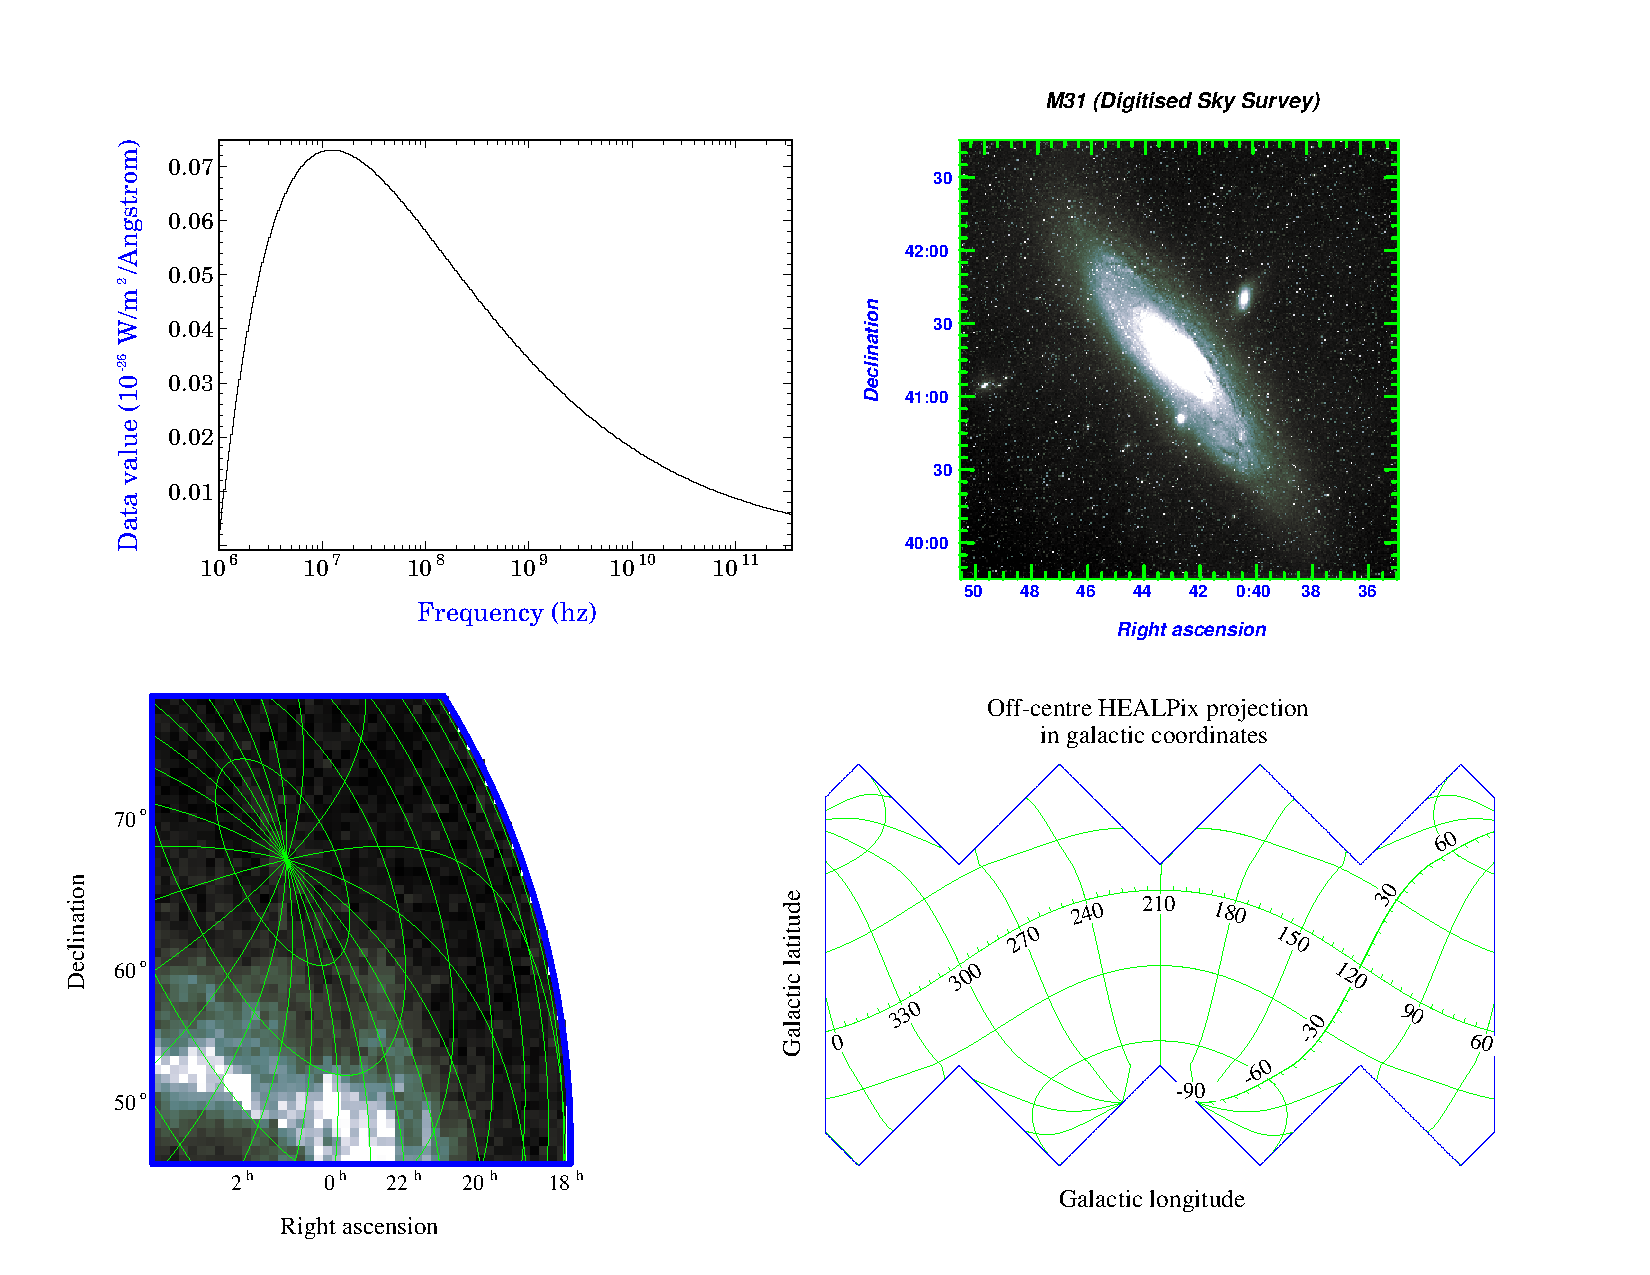
\includegraphics[width=\textwidth]{2dplots}
\caption{A selection of annotated axes created by the Plot class. Note,
Plot only creates the annotated axes --- the background images were
produced using PGPLOT directly. The PGPLOT library was used as the
underlying graphics package for these plots.}
\label{fig:2dplots}
\end{figure*}

\subsubsection{Three Dimensional Plotting}

The \emph{Plot3D} class extends the Plot class to provide plotting
facilities in three dimensions. The basic model is the same as for the
Plot class --- a Plot3D object is a FrameSet in which the base Frame
represents the 3-dimensional Cartesian coordinate system used by the
underlying 3-dimensional plotting package, and the current Frame
represents 3-dimensional ``user'' coordinates.

The projection from 3-dimensional graphics coordinates onto a
2-dimensional plotting surface is handled by the underlying graphics
package. This may be suprising, given that AST could itself handle this
sort of projection. But the decision was taken so that Plot3D graphics
wrapper functions could use the full range of features offered by a
dedicated 3-dimensional plotting packages, rather than restrict it to the
more limited features offered by a typical 2-dimensional package.

Fig.~\ref{fig:3dplot} shows an example of the 3-dimensional annotated axes
produced by Plot3D.

\begin{figure}[h]
\centering
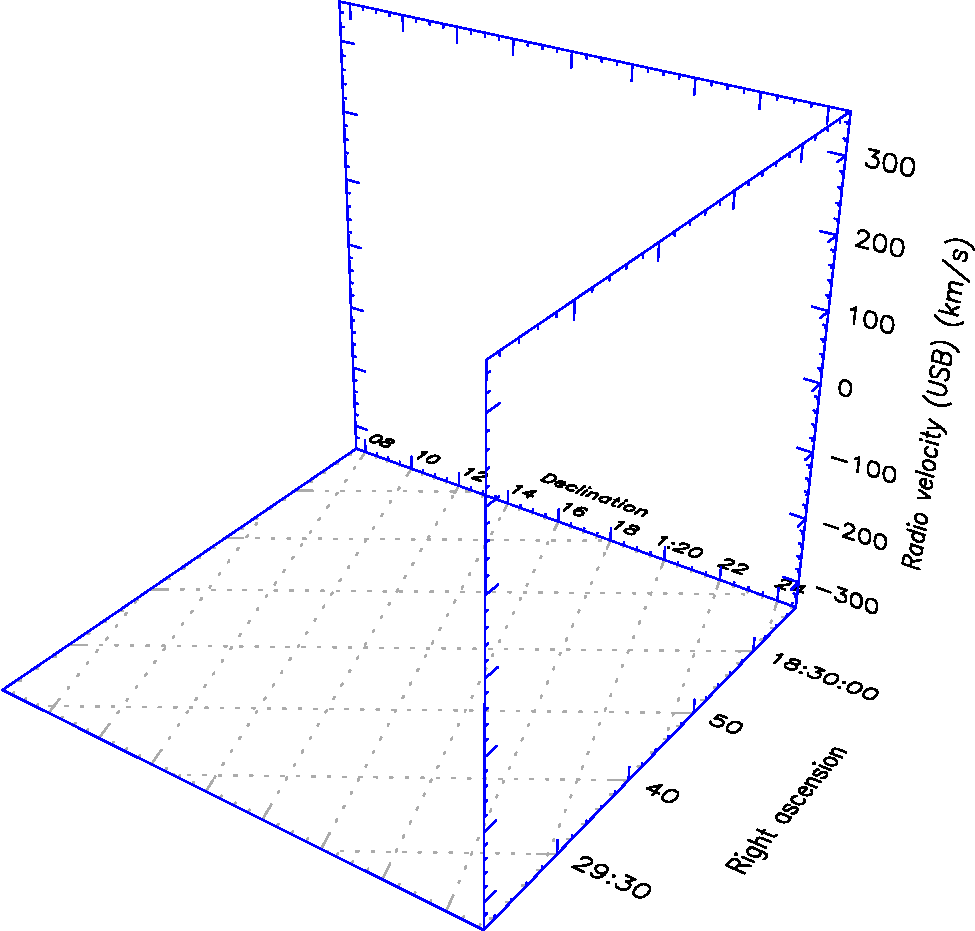
\includegraphics[width=\columnwidth]{3dplot}
\caption{Annotated axes created by the Plot3D class. The 3D interface to the
PGPLOT library included with AST was used as the underlying graphics package
for these plots.}
\label{fig:3dplot}
\end{figure}


\subsection{Flux and Data Unit Transformation}

\subsection{WCS handling}

\subsubsection{Data Resampling and Regridding}





\section{Things we Would do Differently now}

\begin{enumerate}

\item Be clearer about the distinction between a coordinate system and
  a domain. Coordinate systems are mathematical abstractions of
  various types (Cartesian, polar, \emph{etc}). You use a coordinate system
  to describe a position within a physical space (domain). In this
  sense a domain can encapsulate several alternative coordinate
  systems, any of which can be used to describe positions in the
  domain.

\item Have a specific sub-class of Frame to describe a pixel array ( a
  PixelFrame), allowing System=GRID or System=PIXEL.

\item Use degrees instead of radians for sky axes.

\item The restriction that Mappings can only transform doubles may be
  a problem for time axes (but this is an issue with the
  implementation rather than the model).

\item Make it more modular. Some sort of facility for optional
  extensions or plug-ins, so that the thing does not become such a
  huge monolithic lump.

\end{enumerate}

\section{The AST library}

The AST library has been developed over a number of years
\citep{1998ASPC..145...41W,2000ASPC..216..506W,2001ASPC..238..129B,2004ASPC..314..412B,2008ASPC..394..635B,2010ASPC..434..213B,2012ASPC..461..825B}
  and is written in C with no dependencies. It includes code from
  WCSLIB \citep[][\ascl{1108.003}]{2006ASPC..351..591C}, PAL \citep{2013ASPC..475..307J}
  and SOFA \citep[][\ascl{1403.026}]{2011SchpJ...611404H} but does not depend on those
  libraries. There are language bindings for Fortran, Java, Perl and
  Python.

\section{Acknowledgements}

The Starlink software is currently maintained by the Joint Astronomy
Centre, Hawaii with support from the UK Science and Technology
Facilities Council. The source code is open-source using the Lesser
Gnu Public License and is available
online\footnote{\url{https://github.com/Starlink/starlink}}.


%% The Appendices part is started with the command \appendix;
%% appendix sections are then done as normal sections
\appendix

\section{Methods and Properties}
\label{app:classes}

This appendix includes brief descriptions of the more significant methods
and properties of the three main classes used by AST - Mapping, Frame and
FrameSet.

\subsection{The Mapping Class}
The most important public methods of the base Mapping class are:

\begin{description}

\item[astInvert:] Invert a Mapping (i.e. swap the input and output spaces).

\item[astLinearApprox:] Create a new Mapping which is a linear approximation
to the supplied Mapping.

\item[astMapSplit:] Create (if possible) a new Mapping that represents a
subspace within the output space of the supplied Mapping. For instance,
given a Mapping from 3-dimensional pixel coordinates to
(RA,Dec,wavelength), create a Mapping between 2-dimensional pixel
coordinates and (RA,Dec). This is only possible if the requested subspace
is independent of the other output axes.

\item[astRate:] Calculate the rate of change of a specified axis within the
output space, with respect to a specified axis within the input space, at
a given position within the input space.

\item[astRebin:]: Re-bin the pixel values within an input data array to create
an output data array, using the forward transformation of the supplied Mapping
to define the position within the output array at which each input pixel value
is placed.

\item[astResample:]: Re-sample the pixel values within an input data array to
create an output data array, using the inverse transformation of the supplied
Mapping to define the position within the input array from which each
output pixel value is copied. A range of different interpolation schemes
are provided.

\item[astSimplify:] Simplify a compound Mapping (see
section~\ref{sec:simplification}).

\item[astTran:] Transform coordinates using the supplied Mapping.

\end{description}

The most important public properties of the base Mapping class are:
\begin{description}

\item[IsLinear:] A boolean flag indicating if the Mapping is linear.
\item[Nin:] The number of axes within the input space of the Mapping.
\item[Nout:] The number of axes within the output space of the Mapping.
\item[TranForward:] A boolean flag indicating if the Mapping has a defined
forward transformation.
\item[TranInverse:] A boolean flag indicating if the Mapping has a defined
inverse transformation.
\end{description}


%% References
%%
%% Following citation commands can be used in the body text:
%%
%%  \citet{key}  ==>>  Jones et al. (1990)
%%  \citep{key}  ==>>  (Jones et al., 1990)
%%
%% Multiple citations as normal:
%% \citep{key1,key2}         ==>> (Jones et al., 1990; Smith, 1989)
%%                            or  (Jones et al., 1990, 1991)
%%                            or  (Jones et al., 1990a,b)
%% \cite{key} is the equivalent of \citet{key} in author-year mode
%%
%% Full author lists may be forced with \citet* or \citep*, e.g.
%%   \citep*{key}            ==>> (Jones, Baker, and Williams, 1990)
%%
%% Optional notes as:
%%   \citep[chap. 2]{key}    ==>> (Jones et al., 1990, chap. 2)
%%   \citep[e.g.,][]{key}    ==>> (e.g., Jones et al., 1990)
%%   \citep[see][pg. 34]{key}==>> (see Jones et al., 1990, pg. 34)
%%  (Note: in standard LaTeX, only one note is allowed, after the ref.
%%   Here, one note is like the standard, two make pre- and post-notes.)
%%
%%   \citealt{key}          ==>> Jones et al. 1990
%%   \citealt*{key}         ==>> Jones, Baker, and Williams 1990
%%   \citealp{key}          ==>> Jones et al., 1990
%%   \citealp*{key}         ==>> Jones, Baker, and Williams, 1990
%%
%% Additional citation possibilities
%%   \citeauthor{key}       ==>> Jones et al.
%%   \citeauthor*{key}      ==>> Jones, Baker, and Williams
%%   \citeyear{key}         ==>> 1990
%%   \citeyearpar{key}      ==>> (1990)
%%   \citetext{priv. comm.} ==>> (priv. comm.)
%%   \citenum{key}          ==>> 11 [non-superscripted]
%% Note: full author lists depends on whether the bib style supports them;
%%       if not, the abbreviated list is printed even when full requested.
%%
%% For names like della Robbia at the start of a sentence, use
%%   \Citet{dRob98}         ==>> Della Robbia (1998)
%%   \Citep{dRob98}         ==>> (Della Robbia, 1998)
%%   \Citeauthor{dRob98}    ==>> Della Robbia


%% References with bibTeX database:

\bibliographystyle{model2-names-astronomy}
\bibliography{acast}

%% Authors are advised to submit their bibtex database files. They are
%% requested to list a bibtex style file in the manuscript if they do
%% not want to use model2-names.bst.

%% References without bibTeX database:

% \begin{thebibliography}{00}

%% \bibitem must have one of the following forms:
%%   \bibitem[Jones et al.(1990)]{key}...
%%   \bibitem[Jones et al.(1990)Jones, Baker, and Williams]{key}...
%%   \bibitem[Jones et al., 1990]{key}...
%%   \bibitem[\protect\citeauthoryear{Jones, Baker, and Williams}{Jones
%%       et al.}{1990}]{key}...
%%   \bibitem[\protect\citeauthoryear{Jones et al.}{1990}]{key}...
%%   \bibitem[\protect\astroncite{Jones et al.}{1990}]{key}...
%%   \bibitem[\protect\citename{Jones et al., }1990]{key}...
%%   \harvarditem[Jones et al.]{Jones, Baker, and Williams}{1990}{key}...
%%

% \bibitem[ ()]{}

% \end{thebibliography}

\end{document}

%%
%% End of file `elsarticle-template-2-harv.tex'.
